
We estimate the total luminosity of all galaxies below the detection
limit of $z_{850} = 24.72$ using a \citet{schechter76a}
luminosity function, which gives the number of galaxies in the
luminosity interval $[L,L+dL]$ in a given sample,
\begin{equation}
\Phi(L)dL = \Phi^\ast (L/L^\ast)^\alpha e^{-L/L^\ast} d(L/L^\ast).
\end{equation}
$\Phi^\ast$ is a normalization, $L^\ast$ is a
characteristic galaxy luminosity, and $\alpha$ is a unit-less
constant. The ratio of total to observed luminosity is then
\begin{equation}
C = \frac{\int_0^\infty L\Phi(L)dL}{\int_{L_{lim}}^\infty L\Phi(L)dL},
\end{equation}
and we multiply each observed cluster luminosity by C to get the total
luminosity. 

We assume values for $L^\ast$ and $\alpha$ determined in other studies
and use our data to perform a rough consistency check. For $\alpha$,
studies have shown that the value does not evolve much from low
redshift, at least for redder galaxies. Analyzing only red galaxies in
28 clusters spanning $0 < z < 1.3$, \citet{andreon08a} find $\alpha =
-0.91 \pm 0.06$ (rest-frame $V$-band) with no discernible trend in
redshift \citep[see also][]{andreon06a,andreon06c}. From five
intermediate-redshift clusters ($0.54<z<0.9$), \citet{crawford09a}
find a somewhat flatter faint-end slope $\alpha \sim -0.6$ (rest-frame
$B$-band) for the red-sequence luminosity function. Looking at the
full luminosity function, \citet{goto05a} find $\alpha = -0.82 \pm
0.10$ in one cluster at $z=0.83$ (rest-frame $B$-band), compared to
$\alpha = -1.00 \pm 0.06$ in 204 low-redshift clusters (rest-frame
$g$-band) \citep{goto02a}. In redder bands, \citet{strazzullo06a} find
$\alpha \sim -1$ for three clusters at redshifts $1.11 < z < 1.27$ (in
approximately rest-frame $z$ band). Summarizing, most studies find a
value consistent with $\alpha \sim -0.9$, and we assume this value in
computing $C$.

%Note that for the majority of our clusters, the observed $z_{850}$
%band corresponds more closely to rest-frame $B$-band than rest-frame
%$U$ band, but that for the highest-redshift clusters in our sample, we
%are observing rest-frame $U$ band. \citet{goto02a} and \citet{goto05a}
%find a steeper faint-end slope ($\alpha \sim -1.3$) in rest-frame $U$
%band for the full cluster luminosity function, due to the dominance of
%blue star-forming galaxies in the UV. There is little evidence of a
%pass-band dependence for the redder
%galaxies \citep[e.g.,][]{goto02a,andreon06b}.  As we are more
%concerned with tracing the light of redder galaxies that dominate the
%cluster stellar mass, we use a constant value of $\alpha = -0.9$
%independent of cluster redshift.

Values for $M^\ast$ are also reported in most of the above-mentioned
studies. Studies of red galaxies find that the variation of $M^\ast$
with redshift is consistent with passive evolution, with $M^\ast$
decreasing towards higher
redshifts \citep{andreon06c,crawford09a}. \citet{crawford09a} find
$M^\ast_B = -21.1$ and $M^\ast_B \sim -21.3$ (with errors of
approximately a half magnitude) for two clusters at redshifts 0.75 and
0.83. $K$-correcting from the observed
$[3.6]$-band, \citet{andreon06c} find $M^\ast_B \sim -21.7$ at $z \sim
1.1$, with approximately 0.5~magnitudes of evolution between $z=0.3$
and $z=1.1$. At lower redshift (considering all
galaxies) \citet{goto02a} find $M^\ast_B \sim -21.6$, compared to
$M^\ast_B \sim -21.0$ for one cluster at $z=0.83$ \citep{goto05a}. On
the basis of these measurements, we assume a value of $M^\ast_B =
-21.7$.

We have checked our assumed $M^\ast_B$ and $\alpha$ for consistency
with our data. With the set of spectroscopically-confirmed cluster
galaxies from our clusters at $z<1.2$, we confirmed that the bright
end of the luminosity function is consistent with $M^\ast_B = -21.7$,
and strongly inconsistent with values outside the range $M^\ast_B =
-21.7 \pm 0.5$. We also determined the luminosity function using a
statistical subtraction of the ``background'' luminosity function from
the GOODS fields (Fig.~\ref{fig:galproperties_lumfunc}), finding
excellent agreement with the assumed $M^\ast_B$ and $\alpha$ values
over the range $-24 < M_B < -19.8$. ($M_B = -19.8$ corresponds to the
detection limit in the highest-redshift clusters.)

%%%%%%%%%%%%%%%%%%%%%%%%%%%%%%%%%%%%%%%
% FIGURE: CLUSTER LUMINOSITY FUNCTION %
%%%%%%%%%%%%%%%%%%%%%%%%%%%%%%%%%%%%%%%
\begin{figure}[tb]
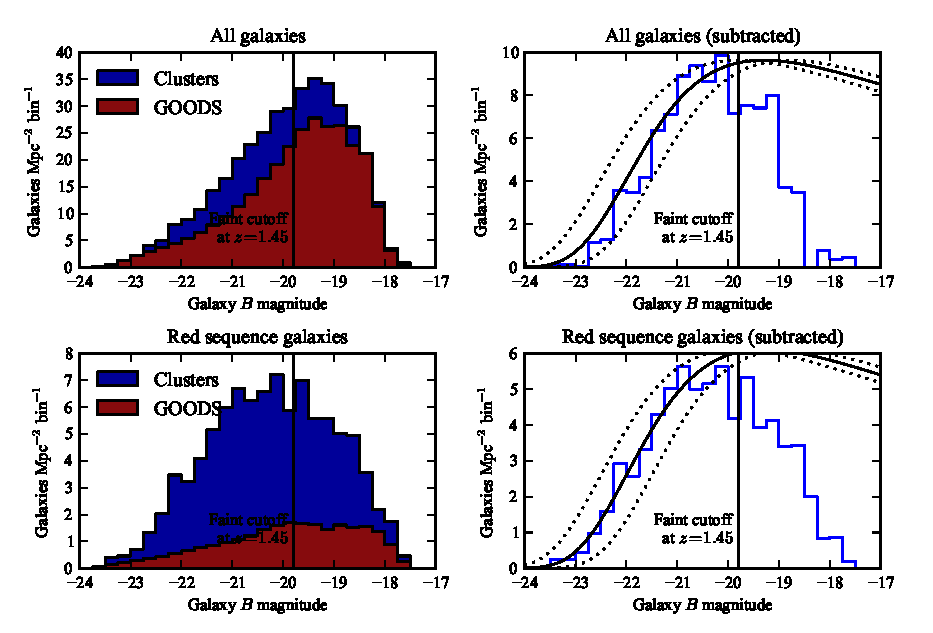
\includegraphics[width=\textwidth]{figures/clrate/galproperties_lumfunc.eps}
\caption[Luminosity function of cluster galaxies]{The luminosity 
function of cluster galaxies (\emph{top panels}) and red-sequence-only
galaxies (\emph{bottom panels}). The \emph{left panels} show the luminosity function
in cluster fields and GOODS fields, showing the clear overdensity in
the cluster fields relative to GOODS. The \emph{right panels} show the
distribution after subtracting the GOODS distribution. The black solid
line shows the luminosity function we assume here ($M^\ast_B = -21.7$,
$\alpha=-0.9$) with dotted lines showing the range used to asses the
systematic uncertainty ($M^\ast_B = -21.7 \pm 0.5$). These
distributions are only reliable to the left of the vertical solid
line, which represents the detection limit in the highest-redshift
cluster.\label{fig:galproperties_lumfunc}}
\end{figure}

For each cluster, we calculate $C$ in the observer frame, converting
$M^\ast_B = -21.7$ to the observed $z_{850}$ band, using the cluster
redshift and a $K$-correction based on a passive galaxy template. In
Table~\ref{tab:lum_params} we report the value $z_{850}^\ast$ and the
resulting correction $C$ for each cluster. The correction is less than
$5\%$ for the majority of clusters, rising to a maximum of 14\% for
the highest-redshift cluster. Because the correction is so small,
varying the assumed values of $M^\ast_B$ and $\alpha$ does not have a
large effect on the total luminosity. Varying $M^\ast_B$ by $\pm
0.5$~mag (a larger range than that allowed by our data) changes the
average correction by only $^{+4}_{-2}\%$. Varying $\alpha$ by $\pm
0.2$ changes the average correction by $^{+5}_{-2}\%$. We
conservatively take $^{+10}_{-3}\%$ (the full range when varying both
concurrently) as the systematic uncertainty in luminosity from the
faint-end correction (summarized in \S\ref{sec:clrate_results_sys}).

%%%%%%%%%%%%%%%%%%%%%%%%%%%%%%%
% luminosity parameters table %
%%%%%%%%%%%%%%%%%%%%%%%%%%%%%%%
\begin{table}[t]
\begin{center}
\caption{\label{tab:lum_params} Bright cutoff magnitudes 
and luminosity function parameters}
\vspace{10pt}
\begin{footnotesizetabular}{lccccc}
\hline
\hline
ID & $z$ & Cutoff from & $z_{850}^{\rm bright}$ & $z_{850}^\ast$ & $C$\\
\hline
A & 1.46 & Max cD & $21.09$ & $22.80$ & $1.143$\\
B & 1.12 & cD & $20.11$ & $21.38$ & $1.033$\\
C & 0.97 & cD & $19.87$ & $20.79$ & $1.018$\\
D & 1.02 & BCG & $20.13$ & $20.95$ & $1.021$\\
E & 1.03 & cD & $19.40$ & $20.99$ & $1.022$\\
F & 1.11 & Max cD & $19.63$ & $21.34$ & $1.031$\\
G & 1.26 & BCG & $20.34$ & $22.04$ & $1.064$\\
H & 1.24 & BCG & $20.33$ & $21.95$ & $1.058$\\
I & 1.34 & Max cD & $20.66$ & $22.37$ & $1.092$\\
J & 1.37 & Max cD & $20.77$ & $22.50$ & $1.104$\\
K & 1.41 & Max cD & $20.92$ & $22.65$ & $1.122$\\
L & 1.37 & Max cD & $20.77$ & $22.50$ & $1.104$\\
M & 0.90 & Max cD & $18.69$ & $20.53$ & $1.014$\\
N & 1.03 & BCG & $20.22$ & $20.99$ & $1.022$\\
P & 1.1\phn & Max cD & $19.58$ & $21.29$ & $1.030$\\
Q & 0.95 & cD & $20.01$ & $20.66$ & $1.015$\\
R & 1.22 & Max cD & $20.15$ & $21.86$ & $1.054$\\
S & 1.07 & Max cD & $19.44$ & $21.16$ & $1.026$\\
T & 0.97 & Max cD & $19.00$ & $20.75$ & $1.017$\\
U & 1.04 & Max cD & $19.31$ & $21.04$ & $1.022$\\
V & 0.90 & cD & $18.89$ & $20.49$ & $1.013$\\
W & 1.26 & Max cD & $20.33$ & $22.04$ & $1.064$\\
X & 1.10 & Max cD & $19.58$ & $21.34$ & $1.031$\\
Y & 1.24 & cD & $20.29$ & $21.90$ & $1.056$\\
Z & 1.39 & cD & $20.85$ & $22.58$ & $1.112$\\
\hline
\end{footnotesizetabular}

\end{center}
{\footnotesize 
{\bf Note.} --- ``Cutoff from'' refers to how $z_{850}^{\rm bright}$ is
determined.  ``cD'': magnitude of visually central dominant
galaxy. ``BCG'': magnitude of visually classified brightest cluster
elliptical (but not central) galaxy. ``Max cD'': Cluster does not have
obvious cD galaxy or clear BCG. In this case, $z_{850}^{\rm bright}$
is $K$-corrected from $M_B = -23.42$, the absolute magnitude of the
brightest cD galaxy in the entire sample.}
\end{table}

